%%
%% memoria.tex
%% 
%\documentclass[a4paper,12pt,titlepage,halfparskip, cleardoubleempty]{scrbook}
\documentclass[a4paper,12pt]{scrbook}
\pagestyle{headings}

\usepackage{tikz}

% Referencias externas
\usepackage{xr-hyper}

%\usepackage[pdftex, breaklinks=false]{hyperref}
\usepackage[pdftex, breaklinks=false, colorlinks=true, linkcolor=black, anchorcolor=black, urlcolor=blue, citecolor=red]{hyperref}

\usepackage[T1]{fontenc}
\usepackage[spanish]{babel}
\usepackage[utf8]{inputenc}

\usepackage[printonlyused]{acronym-custom}

\usepackage{inconsolata}

% Paquete para controlar el interlineado a nivel de entorno
\usepackage{setspace}

%%%%%%%%%%%%%%%
% Paquetes para fuentes

% Paquete para la fuente charter
\usepackage{charter}

% Paquete para la fuente helvética
\usepackage[scaled=0.92]{helvet}

% Paquete para GNUPlot
\usepackage{gnuplottex}

% Guiones de hyphenado
\usepackage{hyphenat}

% Paquete para hacer un índice
\usepackage{makeidx}

% Extra ToC listings
\usepackage{tocbibind}

% Gráficos
\usepackage{graphicx}

% Para poner figuras una al lado de otra
\usepackage[lofdepth,lotdepth]{subfig}

% Paquete para figuras giradas
\usepackage{rotating}

% Automatiza el resaltado de sintaxis usando pygments
\usepackage{minted}

% Cambia el nombre del apéndice de bibliografía
\addto\captionsspanish{
\renewcommand\bibname{Bibliografía y referencias}
}

\makeindex

\begin{document}

\input{ordenes.tex}

% Portada
\begin{titlepage}
  \centering
  \includegraphics[width=.3\textwidth]{logo_uca}

  \bigskip
  \bigskip
  \bigskip
  
%  \begin{changemargin}{3em}{3em}
    \centering

    {\Huge \textsc{\nohyphens{Escuela Superior de Ingeniería}}}
    
    \bigskip
    \bigskip
    \bigskip

    {\huge \nohyphens{Ingeniería Técnica en Informática de Sistemas}}

    \bigskip
    \bigskip
    \bigskip
    \bigskip
    \bigskip
    \bigskip

    {\LARGE \nohyphens{oFlute}}

    \bigskip
    \bigskip
    \bigskip
    \bigskip

    {\large Curso 2009-2010}

    \bigskip
    \bigskip
    \bigskip
    \bigskip
    \bigskip
    \bigskip
    \bigskip
      
%  \end{changemargin}

  {\Large José Tomás Tocino García \\}
  {\large Cádiz, \today}

\end{titlepage}

\cleardoublepage

% Segunda portada
{
  \thispagestyle{empty}
  \centering
  \includegraphics[width=.2\textwidth]{logo_uca}

  \bigskip
  \bigskip
  \bigskip
  
  \begin{changemargin}{3em}{3em}

    \begin{center}
      {\Huge \textsc{\nohyphens{Escuela Superior de Ingeniería}}}
      
      \bigskip
      \bigskip
      
      {\huge \nohyphens{Ingeniería Técnica en Informática de Sistemas}}
      
      \bigskip
      \bigskip
      \bigskip
      \bigskip
      
      {\LARGE \nohyphens{\nombreProyecto}}

\marginpar{Añadir nombre completo}
      
      \bigskip
      \bigskip
      \bigskip
      \bigskip
      
    \end{center}
  \end{changemargin}
  \begin{changemargin}{3em}{1em}
  \begin{flushleft}
    \Large

    \textsc{Departamento}: \nohyphens{Lenguajes y Sistemas Informáticos.} \\
    \textsc{Director del proyecto}: \nohyphens{Manuel Palomo Duarte.} \\
    \textsc{Autor del Proyecto}: \nohyphens{José Tomás Tocino García}. \\
  \end{flushleft}

  \end{changemargin}  

  \bigskip
  \bigskip
  \bigskip
  
  \begin{flushright}
    \large
    Cádiz, \today

    \bigskip
    \bigskip
    \bigskip
    \bigskip    
    \bigskip
    \bigskip

    Fdo.: José Tomás Tocino García
    
  \end{flushright}

}


\cleardoublepage
\bigskip
\bigskip

Este documento se halla bajo la licencia \ac{FDL}. Según estipula la
licencia, se muestra aquí el aviso de copyright. Se ha usado la
versión inglesa de la licencia, al ser la única reconocida
oficialmente por la \ac{FSF}.

\begin{quote}
  Copyright \copyright  2011 José Tomás Tocino García.
  
  Permission is granted to copy, distribute and/or modify this document
  under the terms of the GNU Free Documentation License, Version 1.2
  or any later version published by the Free Software Foundation;
  with no Invariant Sections, no Front-Cover Texts, and no Back-Cover Texts.
  A copy of the license is included in the section entitled "GNU
  Free Documentation License".
\end{quote}

\cleardoublepage

\section*{Agradecimientos}
Quiero agradecer y dedicar la presente memoria y, por extensión, el proyecto
oFlute al completo:
\begin{itemize}
\item A Julian Raschke por crear y mantener Gosu.
\item A Manuel Palomo Duarte y Rafael Rodríguez Galván, de la OSLUCA, por confiar en mí
  como becario de la oficina, apoyarme y darme facilidades para desarrollar el
  proyecto durante la beca.
\item A Antonio García Domínguez, como co-tutor del proyecto, por sus acertados
  consejos, su visión para descubrir cosas mejorables y su implicación con el
  software y el conocimiento libre, gracias a la cual esta memoria fue posible.
\item A mis compañeros más cercanos de la carrera, que me han apoyado y de los
  que me he nutrido para desarrollar este proyecto.
\item A mi familia y mi pareja, que finalmente no tendrán que recibir como
  excusa el desarrollo del proyecto a la hora de dedicarles el tiempo que se
  merecen.
\item A Robert Penner por su magnífico conjunto de ecuaciones para animaciones,
  sin las que oFlute tendría una interfaz mucho más pobre.
\item A los que apuestan por el software libre y el conocimiento abierto. Sus
  herramientas, bibliotecas y documentos han hecho posible que oFlute llegase a
  buen puerto.
\end{itemize}


\cleardoublepage

\tableofcontents
\listoffigures
%\listoftables

\setlength{\parskip}{1.2ex plus 0.4ex minus 0.1ex}
%\setlength{\parskip}{1.2ex}

\chapter{Introducción}
\label{chap:introduccion}
\input{1_introduccion/texto_introduccion.tex}

\chapter{Desarrollo del calendario}
\label{chap:calendario}
\input{2_calendario/texto_calendario.tex}

%\chapter{Descripción general del proyecto}
%
\section{Perspectiva del producto}

\section{Funciones}

Lista de funciones

\section{Características de los usuarios}

\section{Restricciones generales}

\section{Suposiciones y dependencias}


\section{Requisitos para futuras versiones}








 
\chapter{Fundamentos}
\label{chap:fundamentos}
\input{3_investigacion/texto_investigacion.tex}

\chapter{Análisis}
\label{chap:analisis}
\input{4_analisis/texto_analisis.tex}

\chapter{Diseño}
\label{chap:diseno}
En este capítulo se presentarán los detalles de diseño del proyecto, basándonos
en el análisis mostrado en el capítulo anterior. El modelo de clases de diseño
representado aquí es más fiel a la implementación final que el diagrama de
clases conceptuales, pero aún así hay detalles que no se han contemplado por ser
demasiado cercanos a los detalles de implementación.

También en el presente capítulo se detallarán las decisiones de diseño en
relación al aspecto visual de la aplicación, extendiéndonos en el proceso de
creación del logotipo del juego así como de la interfaz gráfica de usuario.

\section{Diagrama de clases de diseño}

Tras la fase de diseño, componían el sistema más de 40 clases, por lo que hemos
tenido que dividir los diagramas en varias partes, intentando seguir cierto
criterio a la hora de elegir qué clases formarán parte de cada división.

En todos los diagramas aparecen, en aras de mantener el contexto, las clases
básicas de la aplicación: \textit{Juego} y \textit{Estado}. Además, hay algunas
otras clases que también se repetirán entre diagramas por conveniencia.

\begin{itemize}
\item En el primer diagrama (figura~\ref{diagrama_clases_1}) aparecen las clases
  relacionadas con el \textit{menú principal}, clases de utilidades (logging y
  animación), y clases para representar elementos gráficos.
\item En el segundo diagrama (figura~\ref{diagrama_clases_2}) aparecen las
  clases relacionadas con el subsistema de análisis del audio, así como las
  secciones \textit{Analizador de Notas} y \textit{Calibrar micrófono}.
\item En el tercer diagrama (figura~\ref{diagrama_clases_2}) aparecen todas las
  clases relacionadas con la sección de \textit{Canciones}.
\item En el cuarto y último diagrama (figura~\ref{diagrama_clases_2}) aparecen
  las clases relacionadas con el motor de \textit{lecciones}.
\end{itemize}

\begin{figure}[htp!]
  \centering
  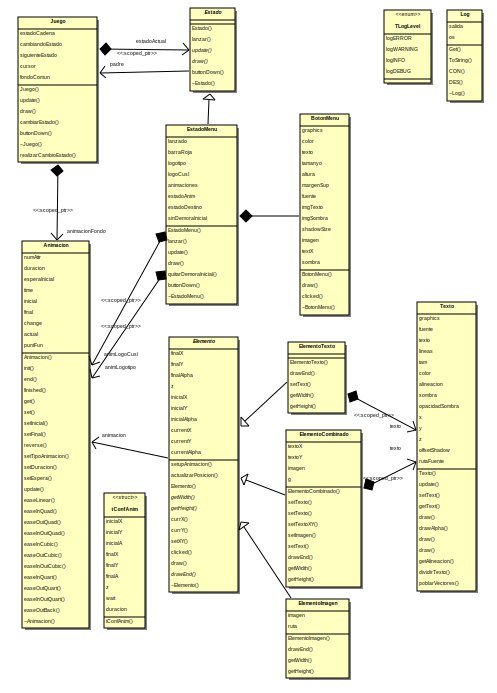
\includegraphics[width=\textwidth]{5_diseno/diagrama1}
  \caption{Diagrama de clases de diseño, parte I}
  \label{fig:diagrama_clases_1}
\end{figure}

\begin{figure}[htp!]
  \centering
  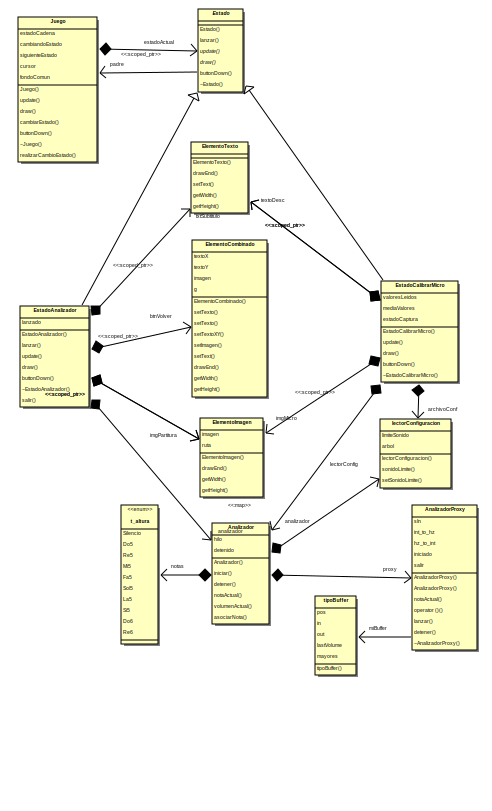
\includegraphics[width=\textwidth, clip=true, trim=0cm 3.5cm 0cm 0cm]{5_diseno/diagrama2}
  \caption{Diagrama de clases de diseño, parte II}
  \label{fig:diagrama_clases_2}
\end{figure}

\begin{figure}[htp!]
  \centering
  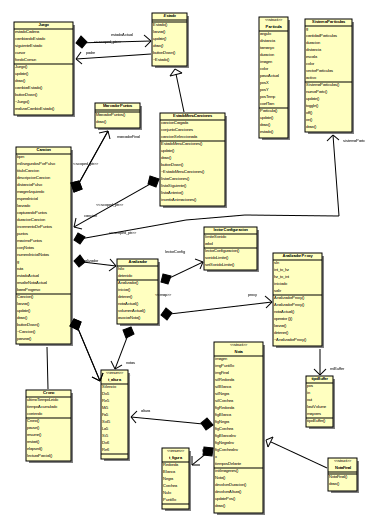
\includegraphics[width=\textwidth, clip=true, trim=0cm 0cm 0cm 0cm]{5_diseno/diagrama3}
  \caption{Diagrama de clases de diseño, parte III}
  \label{fig:diagrama_clases_3}
\end{figure}

\begin{figure}[htp!]
  \centering
  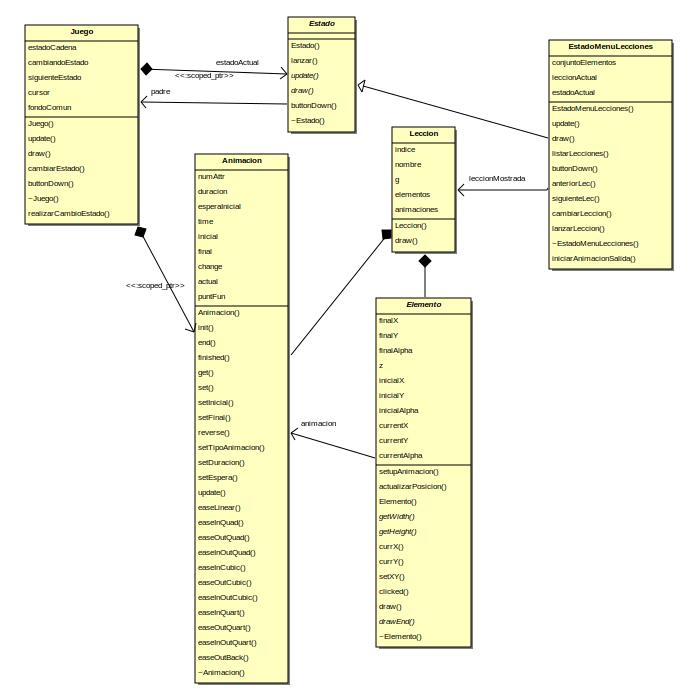
\includegraphics[width=\textwidth, clip=true, trim=0cm 0cm 0cm 0cm]{5_diseno/diagrama4}
  \caption{Diagrama de clases de diseño, parte IV}
  \label{fig:diagrama_clases_4}
\end{figure}

%%% Local Variables: 
%%% mode: latex
%%% TeX-master: "../memoria"
%%% End: 


\chapter{Implementación}
\label{chap:implementacion}
Un análisis claro y un diseño conciso no garantizan que, a la hora de
implementar el sistema planteado, no se encuentre ninguna dificultad o
imprevisto. Así pues, en este capítulo comentaremos los retos y detalles que más
relevancia o complejidad han presentado durante la fase de la implementación del
proyecto.

De igual modo, durante el desarrollo de la aplicacíon se mantuvo actualizada una
bitácora, accesible en línea~\cite{ofluteblog}, en la que se fueron detallando,
a medida que aparecían, muchas de estas dificultades.

Como complemento a la lectura de este capítulo se recomienda tener una copia
local del repositorio del proyecto, disponible para su libre descarga desde la
forja oficial~\cite{ofluteforja}. En él se encuentra todo el código fuente
original, así como la documentación en formato \textit{Doxygen}.

\section{Carga y uso de fuentes TrueType en Gosu}

Como se ha comentado previamente, \textbf{oFlute} hace uso de la biblioteca
\textit{Gosu}, que proporciona una API sencilla para el acceso al sistema
gráfico, entre otras características. Este framework funciona en sistemas
Windows, GNU/Linux y Mac OS, aunque dada la dificultad de conseguir la
compatibilidad con todos ellos, la calidad y el rendimiento es bastante
desigual de un sistema a otro.

Una de estas desigualdades se presentaba a la hora de \textbf{cargar fuentes}
para mostrar textos. En su versión para GNU/Linux, el módulo para el pintado de
textos de Gosu (que comprende la clase \texttt{Gosu::Font} y las funciones
\texttt{Gosu::drawText} y \texttt{Gosu::createText}) solo permitía
utilizar fuentes que estuvieran ya instaladas en el sistema de forma global, de
modo que era imposible adjuntar un fichero con una fuente en formato
\texttt{TrueType}~\cite{reftruetype} para su carga en el juego. 

La instalación de fuentes en sistemas GNU/Linux siempre ha sido una operación
engorrosa que ha requerido permisos de administrador. Esto, unido a que tanto en
Windows como en Mac OS la opción de cargar fuentes desde un fichero sí estaba
disponible, supuso un grave problema en el planteamiento del proyecto.

Inicialmente se investigaron las razones de esta limitación. Al ser un proyecto
libre y abierto, revisamos el código de Gosu, concretamente la implementación
de la clase \texttt{Gosu::Font} previamente citada, de la que dependían todas
las otras funciones relacionadas con fuentes.

Las conclusiones que se sacaron fueron que Gosu, bajo GNU/Linux, implementaba el
renderizado de fuentes mediante una biblioteca llamada Pango~\cite{Pango}, de
bastante bajo nivel, y que por diseño está limitada al uso de fuentes de
sistema, ya que se orienta a herramientas del sistema operativo, no a
aplicativos de terceros.

Así pues, era necesario buscar una alternativa. En numerosos proyectos
previos~\cite{robinson} se había utilizado la biblioteca
\textbf{SDL}~\cite{refsdl}, un framework multimedia muy utilizado en
aplicaciones de audio, vídeo y juegos. Uno de los subsistemas que proporciona
SDL es \textbf{SDL\_ttf}~\cite{refsdlttf}, una biblioteca para el renderizado de
fuentes basadas en ficheros \texttt{truetype}. Esto, unido a que la propia SDL
ya era una dependencia de Gosu, propició que se iniciara la implementación de
una solución basada en este medio.

\subsection{Funcionamiento de \texttt{SDL\_ttf}}

Para comprender cómo se implementó la solución al problema citado, el primer
paso es entender cómo funciona la biblioteca \texttt{SDL\_ttf} para poder ver
cómo se corresponde luego con Gosu.

\subsubsection{Tipos de datos utilizados}

En común con cualquier otra parte del conjunto de partes de SDL, SDL\_ttf se basa
en un tipo de datos conocido como \textit{superficies}
(\texttt{SDL\_Surface}). Estas superficies representan mapas de bits cargados en
memoria, y se utilizan para guardar las imágenes que se cargan de los ficheros,
así como para representar otros destinos gráficos intermedios, como la propia
pantalla.

Para representar el color del texto que vamos a pintar, SDL\_ttf utiliza la
estructura \texttt{SDL\_Color}, que guardará los valores de color de 8 bits para
cada uno de los canales.

Además, SDL\_ttf define un tipo de datos propio, de nombre \texttt{TTF\_Font}, que
representa una fuente cargada a partir de un fichero, con un tamaño determinado.

\subsubsection{Funciones utilizadas}

SDL\_ttf precisa de una \textbf{inicialización} previa, que se lleva a cabo mediante la
llamada a \texttt{TTF\_Init()}. Igualmente, liberaremos los recursos ocupados
mediante \texttt{TTF\_Quit()}.

Para \textbf{cargar la fuente} a partir de los ficheros TrueType (con extensión
\texttt{.ttf}), se utiliza la función \texttt{TTF\_OpenFont(const char * fichero,
  int tamaño)}. Esta función recibe una cadena con el nombre del fichero y el
tamaño de letra a utilizar, y devuelve un puntero al tipo \texttt{TTF\_Font}.

\begin{minted}{cpp}
  TTF_Font * fuente = TTF_OpenFont("fichero_fuente.ttf", 25);
\end{minted}

Una vez cargada la fuente de nuestro interés, tendremos que \textbf{generar una
  superficie} con el texto que queramos. Para ello, SDL\_ttf ofrece una gran
variedad de funciones, según el suavizado del texto y el tipo de caracteres que
estemos utilizando. En nuestro caso, queríamos que la superficie tuviera fondo
transparente, así como usar caracteres en UTF-8\cite{refutf8}, por lo que la
función que se eligió fue 
\begin{minted}{cpp}
  SDL_Surface * TTF_RenderUTF8_Blended (TTF_Font * fuente,
                                        const char * texto,
                                        SDL_Color color);
\end{minted}

Esta función devolverá un puntero a una superficie que se integrará
(\textit{blends}) sobre cualquier imagen, al tener el fondo transparente.


\subsection{Representación de imágenes en Gosu}

Una vez conocidos los tipos de datos y funciones que ofrece SDL\_ttf, es
necesario conocer cuáles son los tipos de datos equivalentes en Gosu, de forma
que pueda haber una \textit{conversión} de un tipo a otro.

\subsubsection{Mapas de bits de bajo nivel: Gosu::Bitmap}
La clase \texttt{Gosu::Bitmap} representa, en Gosu, un mapa de bits de bajo
nivel. Éste no contará con aceleración por hardware ni podrá mostrarse en
pantalla, pero podremos acceder directamente a los datos de los píxeles y
trabajar con ellos.

\texttt{Gosu::Bitmap} nos servirá de paso intermedio entre la superficie de SDL y las
imágenes habituales de Gosu.

\subsubsection{Imágenes de uso común: Gosu::Image}
En Gosu las imágenes y assets gráficos se manejan habitualmente con la clase
\texttt{Gosu::Image}, que representa un contenedor de más alto nivel que
\texttt{Gosu::Bitmap}, además de estar optimizado y poder pintarse en pantalla.

Podremos crear un objeto de esta clase a partir de un \texttt{Gosu::Bitmap}, consiguiendo
finalmente un objeto \textit{pintable}.


\subsection{Implementación final}

Conocidas las representaciones internas de ambas bibliotecas, la implementación
final fue una clase con una interfaz similar a \texttt{Gosu::Font}, de modo que
la transición pudiera ser lo más transparente posible, de nombre
\texttt{CustomFont}.

En el constructor de la se inicializa (de forma única, mediante una variable
estática) el subsistema \texttt{SDL\_ttf} utilizando la llamada
\texttt{TTF\_Init()}. Después, se carga la fuente indicada por los parámetros
del constructor. En ambos casos, se comprueba que el procedimiento ha sido
correcto, lanzando una excepción en caso contrario.

\begin{minted}{cpp}
static int initResult = TTF_Init();
if (initResult < 0)
   throw std::runtime_error("Could not initialize SDL_TTF");

font = TTF_OpenFont(fontName, fontHeight);
if (!font)
   throw std::runtime_error("Could not open TTF file " + fontName);

\end{minted}

Seguidamente, en el método de pintado (\texttt{draw}) se genera la superficie
con el texto que se indique, pasando el contenido de los píxeles a un contenedor
\texttt{Gosu::Bitmap} y finalmente generando un objeto \texttt{Gosu::Image} a
partir del mismo.

\begin{minted}{cpp}
SDL_Surface * surf = TTF_RenderUTF8_Blended(font, text, color);
if (!surface)
   throw std::runtime_error("Could not generate the surface");

Gosu::Bitmap temp;
temp.resize(surf.width(), surf.height());
std::memcpy(temp.data(), surf.data(), temp.width() * temp.height() * 4);

Gosu::Image image (graphic_target, temp);
image.draw(x, y, z);
\end{minted}

\subsection{Recepción}

Una vez contamos con una implementación funcional de la clase, se presentó el
parche en el foro oficial de Gosu~\cite{foroGosu}. En poco tiempo, el
desarrollador principal verificó el código propuesto e hizo una adaptación al
propio código original de la clase \texttt{Gosu::Font} para añadir la
propuesta. 

Por ende, desde la versión \textbf{RELLÉNAME}, el \textit{parche} forma parte
oficial de Gosu, y así se hace indicar en el fichero \texttt{TextUnix.cpp} de la
distribución oficial:

\begin{minted}{cpp}
// [...]

// Used for custom TTF files
// Adapted from customFont class by Jose Tomas Tocino Garcia (TheOm3ga)
class SDLTTFRenderer : boost::noncopyable

// [...]
\end{minted}

Así pues, dado que la solucíon propuesta se integró en la distribución oficial,
nos deshicimos de la clase \texttt{customFont} a favor de la actualización de
\texttt{Gosu::Font}, dado que al fin y al cabo el funcionamiento interno es
el mismo.

\section{Animaciones dinámicas}

Una de las decisiones iniciales de diseño fue la de hacer la interfaz gráfica de
usuario lo más atractiva posible, intentando utilizar gráficos amigables y, en
la medida de lo posible, animaciones y efectos dinámicos.

Con esto, se tornaba necesario crear un sistema de animaciones lo más versátil
posible, de forma que dotar a los elementos de la interfaz de movimiento fuera
un proceso sencillo. 

\subsection{Antecedentes: animaciones en Flash}
Para evitar reinventar la rueda y tener una base estable con la que empezar, se
investigaron sistemas de animaciones ya existentes, evaluando diferentes
enfoques y aproximaciones, sobre todo en sistemas altamente relacionados con las
animaciones. En particular, nos centramos en Adobe Flash (\textit{anteriormente
  Macromedia Flash}) y la gran cantidad de código disponible relacionado con la
generación de animaciones dinámicas.

Especialmente interesante es el trabajo de Robert Penner, un programador
americano muy interesado en la programación matemática, que ideó un sistema de
animaciones dinámicas para ActionScript~\cite{actionscript} 1.0 y 2.0. Penner,
en su libro \textit{Programming Macromedia Flash MX}~\cite{libropenner} incluyó
un capítulo llamado \textit{Motion, Tweening and Easing} (que dada su
popularidad acabó ofreciendo de forma gratuita~\cite{capitulopenner}), en el que
por primera vez presentó y explicó con detalle su sistema de animaciones.

En el citado capítulo se desgranan las animaciones como ecuaciones dependientes
del tiempo y de las posiciones inicial y final, de forma que fuera fácil generar
una serie de funciones para determinar la posición de un objeto en cada
instante. Una vez presentados los conceptos iniciales, Penner desvela una serie
de ecuaciones de movimiento (que acabaron siendo bautizadas y mundialmente
conocidas como las \textit{Penner's Easing Equations}). Estas ecuaciones modelan
un gran número de movimientos, en función de cómo varía la posición respecto del
tiempo (y perceptualmente la aceleración/deceleración del objeto animado).

Además, por cada tipo de ecuación, Robert Penner generó tres tipos de
movimientos: de aceleración (\textit{ease in}), de deceleración o frenada
(\textit{ease out}), y de aceleración-deceleración (\textit{ease in-out}). Con
esto, quedaban cubiertas la práctica totalidad de los tipos de animaciones posibles.

Así, un ejemplo de ecuación podrían ser las cúbicas, que hacen que la posición
del movimiento se rija por una función cúbica del tiempo. Si graficamos la
relación del tiempo por la posición, ambos de 0 a 1, el resultado sería el
siguiente:

{\Large\textbf{GRÁFICA x*x*x}}

Tras estudiar bien el código original, se decidió hacer una adaptación en C++,
de forma que se adaptara a las necesidades del proyecto.

\subsection{Adaptación en C++}
El primer paso fue portar las ecuaciones propiamente dichas -- esto es, las
funciones que generaban las posiciones intermedias. Dado que el lenguaje
original, ActionScript, es un derivado de EcmaScript~\cite{Ecmascript}, la
sintaxis es prácticamente idéntica a C++ en cuanto a asignaciones y operadores
se refiere, por lo que este paso fue prácticamente transparente.

Seguidamente, se ideó un \textit{wrapper} para estas ecuaciones, de forma que
fuera un objeto independiente el que se encargara de calcular las posiciones
intermedias de la animación, en lugar de tener que hacerlo los propios objetos
animados. Para ello, se creó la clase \texttt{Animación}, con las siguientes
características:
\begin{itemize}
\item Para cada instancia, permite animar un número arbitrario de valores, de
  forma que con un solo objeto \textit{Animacion} podamos animar la posición
  horizontal y vertical de un objeto, por ejemplo.
\item Permite elegir entre tres tipos de movimiento (\textit{ease in},
  \textit{ease out} y \textit{ease in-out}) para tres ecuaciones distintas
  (cuadrática, cúbica y cuártica), además de una ecuación especial con
  movimiento de ida y vuelta, y, lógicamente, movimiento uniforme. En total, 11
  posibles movimientos.
\item Capacidad para atrasar las animaciones, de forma que sea sencillo generar
  animaciones escalonadas de varios elementos sin tener que recurrir a
  \textit{callbacks}.
\end{itemize}

\subsection{Ejemplo de uso}

Supongamos que tenemos una pelota que queremos mover diagonalmente con un
movimiento de aceleración, desde la posición 0,0 hasta la posición 150, 300, en
30 pasos. Además, tenemos un cuadrado que habrá de moverse de la posición 0, 150
hasta la posición 150,150 cuando la pelota vaya por la mitad de su camino, y que
llegue a la vez que aquella.

Para cumplir este objetivo, crearemos dos objetos \texttt{Animación}, uno para
la pelota y otro para el cuadrado. En el caso de la pelota estaremos animando
dos parámetros, la posición horizontal y la vertical, y la duración será de 30
pasos. El tipo de movimiento será de aceleración, y la ecuación que elegiremos
será la cuadrática. Al no indicarse nada, no habrá espera inicial.

\begin{minted}{cpp}
// Creamos la instancia
Animacion animPelota (2, 30, Animacion::tEaseInQuad, 0);

// Asignamos la pos inicial y final de la coordenada horizontal
animPelota.set(0, 0, 150);  

// Coordenada vertical
animPelota.set(1, 0, 300);
\end{minted}

En el caso del cuadrado el movimiento sólo será horizontal, por lo que
animaremos un parámetro. Además, el movimiento comenzará cuando la anterior
animación vaya por la mitad (esto es, en el paso 15), y deberá llegar a la vez,
por lo que la duración será de 15 pasos.

\begin{minted}{cpp}
// Creamos la instancia de la clase
Animacion animCuadrado (1, 15, Animacion::tEaseInQuad, 15);

// Asignamos las posiciones inicial y final
animCuadrado.set(0, 0, 150);
\end{minted}

Una vez inicializados los objetos \texttt{Animación}, tendremos que hacer que,
en cada iteración del bucle de juego, las animaciones se actualicen. Para ello,
la clase \texttt{Animación} dispone de un método \texttt{update}. Además,
haremos uso del método \texttt{get} para obtener las posiciones intermedias y
así actualizar el objeto

\begin{minted}{cpp}
// ...
// En la fase update del bucle de juego
animPelota.update();
animCuadrado.update();

imagenPelota -> draw(animPelota.get(0), animPelota.get(1));
imagenCuadrado -> draw(animCuadrado.get(0), 150);
\end{minted}

Con esto, ya estará lista la animación de ambos objetos. De cualquier modo, la
clase \texttt{Animación} provee otros métodos que pueden resultar de interés,
como el método \texttt{finished}, que comprueba si las animaciones han
concluído. 

Además, las ecuaciones de los movimientos han sido implementadas en forma de
funciones estáticas, por lo que es posible acceder a las mismas para hacer
cálculos puntuales si fuera necesario. En tal caso, hay que tener en cuenta que
todas las ecuaciones reciben cuatro parámetros, estos son, en orden:

\begin{itemize}
\item Tiempo transcurrido.
\item Valor inicial del atributo a animar.
\item \textit{Delta} del atributo en la animación (final - inicial).
\item Duración de la animación en pasos.
\end{itemize}

Con esto, será posible controlar las animaciones de forma independiente, sin
necesidad de crear una instancia de la clase.




\chapter{Pruebas}
\label{chap:pruebas}
En este capítulo se detallan las pruebas a las que se ha sometido
\textbf{oFlute}. Habitualmente, probar un videojuego o aplicación con gran
interactividad suele ser un proceso complejo. Dada la gran cantidad de
situaciones distintas que pueden tener lugar, es difícil recrear y probar todos
los escenarios posibles. Tanto es así que, en los grandes equipos de desarrollo,
hay empleados que se dedican al completo a probar los productos.

En oFlute, las pruebas se han organizado al final de cada iteración, comprobando
el correcto funcionamiento de cada nueva funcionalidad, por separado, y luego
integrando el conjunto. Además, ciertos módulos no asociados a iteraciones (como
el sistema de animaciones (sección \ref{sec:animaciones}) también fueron
probados de manera independiente.

\section{Pruebas unitarias}
Las \textbf{pruebas unitarias} se encargan de comprobar el correcto
funcionamiento de módulos y fragmentos por separado. En nuestro caso, todos los
módulos fueron probados por separado, utilizando a tal efecto ramas de
desarrollo alternativas que probaban cada funcionalidad en particular. 

\section{Pruebas de integración}

\section{Pruebas de jugabilidad}

\section{Pruebas de interfaz}



\chapter{Conclusiones}
\label{chap:conclusiones}
Durante el transcurso del desarrollo de oFlute, y sobre todo al término del
mismo, se han obtenido unas conclusiones y unos resultados, tanto de forma
personal como para con la comunidad, que intentaremos reflejar en este capítulo.

oFlute ha sido el proyecto más longevo al que me he enfrentado hasta ahora. A
pesar de tener conciencia de la envergadura del mismo desde el principio, el
tiempo para completarlo ha superado todas mis expectativas, sobre todo en lo que
a documentación se refiere. La causa de esto ha sido, por un lado, una
planificación inicial algo ineficiente y, por otro lado, mi recelo sobre los
procedimientos actuales sobre ingeniería del software. De cualquier modo, estoy
bastante satisfecho con lo obtenido, y esto me ha servido para aprender a
regirme por una planificación de forma más estricta.

Gracias a oFlute he aprendido las técnicas básicas de la programación de audio,
sobre todo en la parte técnica más que teórica. Es esta parte teórica, sobre
todo la de análisis, la que me gustaría reforzar en un futuro, ahora que cuento
con las bases para conseguirlo. Como se comentó en el capítulo sobre
\textit{Investigación preliminar}, los videojuegos relacionados con el audio son
un nicho aún poco explorado y que puede dar muchas satisfacciones, sobre todo
cuando el producto se orienta a un público joven.

Por otro lado, oFlute también me ha ayudado a aprender a usar algunas
tecnologías secundarias, en algunos casos incluso obteniendo un conocimiento
suficiente para generar documentación e impartir talleres relacionados con ello.

Una de estas tecnologías es \textbf{Boost}~\cite{boost}, un conjunto de
bibliotecas para C++ que amplían en gran medida la biblioteca estándar del
lenguaje. Un amplio número de componentes de Boost formarán parte del nuevo
estándar C++0x~\cite{cpp0x}, por lo que me ha servido para ponerme al día en las
novedades que están por llegar.

Utilizando como material de apoyo el libro \textit{``Beyond the C++ Standard
  Library''}~\cite{libroboost}, pude conocer una gran parte de las bibliotecas
  de Boost, incluyendo punteros inteligentes, programación funcional,
  bibliotecas para hilos, y utilizarlas en el proyecto. Además, también apliqué
  este nuevo conocimiento en el desarrollo de un taller durante los Cursos de
  Verano de la OSLUCA~\cite{cursosverano}, en el que se explicaron las partes más
  importantes de Boost, con numerosos ejemplos de cada una. Toda la
  documentación es libre~\cite{materialesCursoBoost}.

Al tratarse de la principal biblioteca utilizada durante el desarrollo, oFlute
me ha provisto de un profundo conocimiento de \textbf{Gosu}~\cite{gosu},
permitiéndome implementar videojuegos con mucha más fluidez y labrándome un
pequeño \textit{framework} personal que utilizar de base en próximos
proyectos. A raíz de esto impartí un taller~\cite{tallergosu} sobre la
biblioteca en colaboración con la ADVUCA~\cite{advuca}, cuya
afluencia superó las 50 personas. Los materiales pueden descargarse
libremente~\cite{tallergosumateriales}.

Uno de estos proyectos \textit{``hijos''} de oFlute ha sido
\textbf{Freegemas}~\cite{freegemas}, un clon libre del popular juego tipo puzzle
\textit{Bejeweled}. Freegemas es multiplataforma, funciona tanto en GNU/Linux
como en Windows, y además forma parte oficial de Guadalinex~\cite{guadalinex},
por lo que es posible encontrarlo en los repositorios oficiales. 

\begin{figure}[h!]
  \centering
  \includegraphics[width=0.55\textwidth]{8_conclusiones/imagen_freegemas}
  \caption{Logotipo de Freegemas}
\end{figure}

Además, Freegemas sirvió como base para una serie de tres artículos que
publiqué, junto al doctor Manuel Palomo Duarte, en la revista Linux
Magazine~\cite{linuxmagazine} sobre desarrollo de videojuegos en C++. Es posible
encontrar estos artículos en el archivo de la
revista~\cite{refarticulo1}\cite{refarticulo2}\cite{refarticulo3} bajo una
licencia Creative Commons.

Otra de las tecnologías que he aprendido ha sido \textbf{GNU Gettext}, que ha
servido para internacionalizar el proyecto. A este efecto escribí una guía
concisa sobre traducción de proyectos con esta herramienta, que se puede
encontrar en el apéndice~\textit{\nameref{sec:gettext}}.

Por otro lado, gracias a oFlute tuve la oportunidad de participar en el IV
Concurso Universitario de Software Libre~\cite{cusl}. En el transcurso del
concurso formé parte de una comunidad muy unida, en la que reinó el apoyo y la
ayuda entre los concursantes. La final del concurso se celebró en la Escuela
Superior de Ingeniería de Cádiz, en la que oFlute obtuvo una mención
especial~\cite{cusl2}.

\begin{figure}[h!]
  \centering
  \includegraphics[width=0.65\textwidth]{8_conclusiones/imagen_logocusl}
  \caption{IV Concurso Universitario de Software Libre}
\end{figure}

Previa a la final nacional tuvo lugar la fase local del concurso, en el que el
proyecto también recibió un accésit al mejor proyecto de
innovación~\cite{cusllocal}.


\appendix

\chapter{Herramientas utilizadas}
\label{chap:herramientas}
\input{apendice_herramientas/texto_apendice_herramientas.tex}

\chapter{Manual de instalación}
\label{chap:manual_instalacion}
A continuación se presentan las instrucciones de instalación de \textbf{oFlute}
en sistemas GNU/Linux basados en paquetería Debian\cite{refdebian}, por
ser los que más auge están teniendo en la actualidad. Tomaremos como referencia
la distribución Ubuntu 10.04.3 LTS\cite{refubuntu}.

\section{Instalación de dependencias}

El primer paso a la hora de instalar oFlute es hacernos con las dependencias del
proyecto. Para ello, utilizaremos el gestor \texttt{apt-get}, pero para otros
sistemas el procedimiento será similar.

La instalación de las dependencias se hará con el siguiente comando:

\begin{minted}{bash}
  sudo apt-get install subversion g++ libgl1-mesa-dev libpango1.0-dev \
libboost1.40-dev libsdl-mixer1.2-dev libsdl-ttf2.0-dev \
libboost-serialization1.40-dev libpulse-dev libboost-regex1.40-dev \
libboost-filesystem-dev libboost-thread-dev 
\end{minted}

Aunque pueda parecer que son numerosas, realmente casi todas las dependencias
forman parte de la instalación de Gosu, la biblioteca de desarrollo de
videojuegos 2D. Al no ser una biblioteca lo suficientemente popular, aún no se
encuentra empaquetada en los repositorios de las principales distribuciones, por
lo que se hace necesario instalarla a partir del código fuente.

\section{Descarga del código fuente}

Seguidamente, hemos de hacernos con una copia local del repositorio, que
contiene el código fuente. Al tratarse de un proyecto libre, el repositorio es
de acceso público\cite{ofluteforja}.

Haciendo uso del comando \texttt{svn}, haremos una copia local del repositorio
Subversion\cite{refsubversion} en nuestro sistema con la siguiente orden:

\begin{minted}{bash}
  svn checkout http://oflute.googlecode.com/svn/trunk oflute
\end{minted}

Con ello, se creará una carpeta llamada \texttt{oflute} en la que se encontrarán
los ficheros de la rama principal (\texttt{trunk}) del proyecto.

\section{Compilación}

Como se ha comentado previamente, será necesario compilar la biblioteca Gosu
previamente. Para ello, se ha facilitado un objetivo en el script de compilación
\texttt{Makefile}~\cite{refmakefile} que automatiza el proceso.

Así, el primer paso será, estando en la carpeta recién creada, utilizar el
siguiente comando:

\begin{minted}{bash}
  make libgosu
\end{minted}

Una vez concluida la compilación de Gosu, pasaremos a compilar el propio
proyecto mediante la siguiente orden:

\begin{minted}{bash}
  make
\end{minted}

\section{Configuración del micrófono}
Antes de poder lanzar el juego, será necesario configurar las opciones de audio
del sistema operativo. Por defecto, la entrada de audio suele estar mutada, por
lo que será imposible que la aplicación tenga acceso al sonido proveniente del
micrófono.

Siguiendo con la referencia de Ubuntu, iremos al menú \textit{Sistema}, luego a
\textit{Preferencias} y, finalmente, elegiremos \textit{Sonido}. Una vez ahí,
pasaremos a la pestaña \textit{Entrada} y, en caso de que estuviera marcada,
desmarcaremos la opción \textit{Silenciar}, tal y como muestra la imagen.

\begin{figure}[h!]
  \centering
  \includegraphics[width=0.75\textwidth]{apendice_manual_instalacion/imagen_captura_1}
  \caption{Panel de configuración del micrófono}
\end{figure}

\vspace{-1cm}

\section{Ejecución}

Al término de las anteriores etapas, se habrá generado un ejecutable de nombre
\texttt{oflute}, por lo que será posible lanzar la aplicación a través del
siguiente comando:

\begin{minted}{bash}
  ./oflute
\end{minted}



\chapter{Manual de usuario}
\label{chap:manual_usuario}
En este capítulo se explicará el funcionamiento de la aplicación desde el punto
de vista del usuario final, detallando las opciones de cada una de las secciones.

Para poder acceder a la aplicación, tal y como se explicó en el
\textit{\nameref{sec:mainstalacion}}, será necesario utilizar el comando:

\begin{minted}{bash}
  ./oflute
\end{minted}

\section{Ejecución inicial}
Al lanzar la aplicación, se abrirá una ventana y aparecerán, consecutivamente,
la pantalla de créditos del autor y la pantalla de presentación del
juego. Pasados unos momentos éstas desaparecerán, aunque tiene la opción de
omitir cada una de las pantallas pulsando la tecla \texttt{escape}.

\begin{figure}[h!]
  \centering
  \includegraphics[width=0.8\textwidth]{apendice_manual_usuario/imagen_estadoAutor}
  \caption{Pantalla de créditos del autor}
  \vspace{-1cm}
\end{figure}

\begin{figure}[h!]
  \centering
  \includegraphics[width=0.8\textwidth]{apendice_manual_usuario/imagen_estadoIntro}
  \caption{Pantalla de presentación del juego}
  \vspace{-0.3cm}
\end{figure}

Una vez desaparezcan ambas pantallas, se iniciará una animación para mostrar el
menú principal. Puede cancelar la animación y mostrar rápidamente el menú
principal pulsando la tecla \texttt{escape}.

\begin{figure}[h!]
  \centering
  \includegraphics[width=0.8\textwidth]{apendice_manual_usuario/imagen_menuPrincipal}
  \caption{Pantalla del menú principal}
  \vspace{-1cm}
\end{figure}






\chapter{Manual para añadir nuevas canciones}
\label{chap:manual_canciones}
En \textbf{oFlute} existe la posibilidad de añadir nuevas canciones al juego, de
forma que los usuarios puedan ampliar el juego y que éste se convierta en una
herramienta lúdica prácticamente ilímitada.

Así, en un futuro podrán existir, por ejemplo, packs temáticos de canciones
descargables desde internet, con los que seguir practicando nuestra pericia con
la flauta dulce.

\section{Ficheros necesarios}

Cada una de las canciones presentes en el juego necesitará un fichero donde se
definirán las características y notas de la canción. El nombre de estos ficheros
sigue la estructura \texttt{songN.xml}, donde \textit{N} es el número de canción
a añadir.

Los ficheros de las canciones se encuentran en la carpeta \texttt{canciones},
ubicada en el directorio raíz de la instalación de oFlute. 

\section{Estructura del fichero de canciones}

\subsection{Lenguaje XML}
\label{sec:lenguaje-xml}

Cada fichero de canción es un archivo \textit{XML}. \marginpar{REFERENCIA} XML
son las siglas, en inglés, de \textit{eXtensible Markup Language} -- lenguaje de
marcado extensible. La tecnología XML busca dar solución al problema de expresar
información estructurada de la manera más abstracta y reutilizable posible. 

Para ello, utiliza una serie de \textit{etiquetas}, organizadas de forma
jerárquica, que siguen la forma \texttt{<nombre>}, donde \textit{nombre} es la
identificación del elemento que se está representando. Las etiquetas deben
cerrarse utilizando la sintaxis \texttt{</nombre>}. Entre las etiquetas de
apertura y cierre pueden anidarse otras etiquetas, así como información en
formato texto.

Todo documento XML tiene una etiqueta \textit{raíz}, de la cual cuelgan todas
las demás. En nuestro caso, los ficheros que representan las canciones tendrán
como raíz el elemento \texttt{Song}. Este es un ejemplo de un fichero completo:



\begin{minted}{xml}
<?xml version="1.0" ?>
<Song>
  <Title>Los pajaritos</Title>
  <Desc>Van por el aire</Desc>
  <BPM>60</BPM>
  <Notes>do5n mi5c fa5c sol5n sol5c sol5c la5n la5c la5c sol5n 
   sol5n fa5n fa5n mi5n mi5n re5c mi5c fa5c re5c do5n do5n</Notes>
</Song>
\end{minted}

\subsection{Campos iniciales}

\subsubsection{Título de la canción}

%\usestyle{default}

El título de la canción se indicará mediante la etiqueta \texttt{<Title>}, por ejemplo:

\inputminted{xml}{apendice_manual_canciones/snippet_1}

\subsubsection{Descripción de la canción}

La descripción de la canción sirve como subtítulo de la misma. Se definirá con
la etiqueta \texttt{<Desc>}, por ejemplo:

\inputminted{xml}{apendice_manual_canciones/snippet_2}

\subsubsection{Ritmo}

El ritmo de la canción se define como el número de pulsos por minuto -- en
inglés, \textbf{bpm}, \textit{beats per minute}. Podemos definir este atributo
con la etiqueta \texttt{<BPM>}, por ejemplo:

\inputminted{xml}{apendice_manual_canciones/snippet_3}

\subsection{Definición de las notas}

Ésta es la parte más importante del fichero de definición de canciones. Aquí se
indicarán las notas que queremos que aparezcan en el pentagrama y,
consecuentemente, que el jugador interprete.

Las notas se escribirán dentro de la etiqueta \texttt{<Notes>}, en orden
consecutivo y separadas por un espacio.

\inputminted{xml}{apendice_manual_canciones/snippet_4}

Cada una de las notas deberá representarse según la siguiente expresión
regular:
\begin{verbatim}
(do|re|mi|fa|sol|la|si|xx)(5|6|0)(r|b|n|c)(p)?
\end{verbatim}

La descomposición de esta sintaxis es la que sigue:
\begin{description}
\item[Altura] Se indicará con el texto de la nota (\textit{do}, \textit{re},
  \textit{mi}...) o, en el caso de querer incluir un silencio, con el texto
  \textit{xx}.
\item[Octava] La flauta dulce habitualmente solo cubre desde el Do en la quinta
  octava hasta el Re en la sexta octava. Ésta se indicará con un número, 5 ó 6,
  ó un 0 si estamos incluyendo un silencio.
\item[Duración] Las posibles duraciones son la redonda (4 tiempos), la blanca (2
  tiempos), la negra (1 tiempo) y la corchea (medio tiempo). Para indicar el
  mismo, se usarán las iniciales de los nombres, esto es, \textit{``r''},
  \textit{``b''}, \textit{``n''} o \textit{``c''}.
\item[Puntillo] Es posible añadir puntillo a las notas, incrementando su
  duración en la mitad de su tiempo original. Para ello, incluiremos la letra
  \textit{``p''} al final.
\end{description}

Una vez escritas las notas, ya tendremos el fichero de nuestra canción listo
para ser incluido en oFlute. Un ejemplo de fichero de canción completo podría
ser el siguiente:

\inputminted{xml}{apendice_manual_canciones/snippet_5}

\chapter{Manual para añadir nuevas lecciones}
\label{chap:manual_lecciones}
\textbf{oFlute} fue diseñado de forma que se pudiera expandir de manera
sencilla. Además de poder añadir canciones nuevas tal y como se explicó en el
apéndice \textit{\nameref{chap:manual_canciones}}, también es posible añadir
nuevas lecciones a la aplicación.

\section{Ficheros necesarios}

Las lecciones necesitan de más ficheros que las canciones, ya que se basan en
elementos multimedia para mejorar la experiencia de usuario. Así, una lección
dispondrá de un fichero base en formato XML y de una serie de archivos
auxiliares de recursos. Por ahora, \textbf{oFlute} acepta recursos en formato
imagen PNG~\cite{refpng} y fuentes TTF~\cite{reftruetype}, pero en un futuro
será posible añadir otros tipos de elementos.

\subsection{Fichero de lección}
El fichero base deberá alojarse en el directorio \texttt{lecciones}, dentro de
la carpeta raíz de la instalación de oFlute. Además, su nombre debe seguir la
estructura \texttt{lecN.xml}, donde \textit{N} es el número de la lección a
añadir.

\subsection{Ficheros de recursos}
Los ficheros de recursos podrán guardarse en cualquier lugar dentro de la
carpeta de instalación de oFlute. De cualquier modo, se recomienda guardar las
imágenes en la carpeta \texttt{media/lecciones} y las fuentes en la carpeta
\texttt{media}, ya que es ahí donde están los recursos de las otras lecciones,
facilitando la reutilización.

\section{Estructura del fichero de lección}

Como se comentó en la sección \ref{sec:lenguaje-xml}, todos los documentos XML
necesitan un elemento raíz. En este caso, usaremos la etiqueta \texttt{<Lec>}
como raíz del fichero de lección.


\subsection{Campos iniciales}

\subsubsection{Índice}
Es posible añadir el índice de la lección, de forma que podamos decidir
fácilmente el orden en que aparecerá dentro de la lista de lecciones del sistema.

Para ello, utilizaremos la etiqueta \texttt{<index>}, tal que así:

\inputminted{xml}{apendice_manual_lecciones/snippet_1}

\subsubsection{Nombre}
El nombre de la lección lo añadiremos utilizando la etiqueta
\texttt{<nombre>}. Éste se utilizará en la pantalla de selección de lecciones.

\inputminted{xml}{apendice_manual_lecciones/snippet_2}

\subsubsection{Descripción}

La descripción de la lección nos permitirá conocer brevemente su contenido sin
tener que acceder directamente a la misma. Se empleará la etiqueta
\texttt{<descrip>} para identificar la descripción.

\inputminted{xml}{apendice_manual_lecciones/snippet_3}

\subsection{Elementos multimedia}
Tras los campos iniciales, se indicarán los elementos multimedia. Podremos
encontrar dos tipos: imágenes, cargadas a partir de los ficheros de recursos
previamente comentados, y textos, que se dibujan de forma dinámica. Para ello,
marcaremos una sección con la etiqueta \texttt{<elementos>}.

\begin{minted}{xml}
<elementos>
...
</elementos>  
\end{minted}

Cabe notar que todos los elementos multimedia aparecerán en pantalla mediante
una animación de desvanecimiento o \textit{fade-in}. Para indicar el orden en
que éstos aparecerán, las etiquetas de los elementos multimedia tendrán un
atributo \texttt{wait}, que indica el retraso en el inicio de la animación.

\subsubsection{Imágenes}
Las imágenes se indicarán mediante la etiqueta simple \texttt{<img/>} --
\textit{simple}, porque se cerrará a sí misma, desapareciendo la etiqueta de
cierre posterior.

Esta etiqueta tendrá los siguientes atributos:
\begin{description}
\item[src] Indica la ruta al fichero de imagen, relativa al directorio raíz de
  oFlute.
\item[x, y, z] Posición horizontal, vertical y profundidad del elemento en
  pantalla, en píxeles.
\item[wait] Como se ha comentado, es el retraso en la animación de aparición.
\end{description}

Un ejemplo de definición de elemento multimedia en formato imagen podría ser el
siguiente:

\inputminted{xml}{apendice_manual_lecciones/snippet_4}

\subsubsection{Textos}
Los textos utilizan la etiqueta \texttt{<texto>}. Dentro de la etiqueta, esto
es, entre la etiqueta de apertura \texttt{<texto>} y la de cierre
\texttt{</texto>}, se habrá de escribir el texto que queremos que se
muestre. Hay que tener en cuenta que los saltos de línea que insertemos
aparecerán tal cual posteriormente en pantalla.

Además, la etiqueta consta con numerosos atributos obligatorios:
\begin{description}
\item[tam] Indica el tamaño de la fuente en pantalla.
\item[ca, cr, cg, cb] Para definir el color del texto utilizamos su definición
  RGBA~\cite{rgba} (\textit{Red, Green, Blue, Alpha}), esto es, los
  valores individuales de los canales rojo, verde, azul y alfa (opacidad). Así,
  cada uno de los atributos indica el valor de un canal:
  \begin{description}
  \item[ca] Canal alfa.
  \item[cr] Canal rojo.
  \item[cg] Canal verde.
  \item[cb] Canal azul.
  \end{description}
\item[x, y, z] Definen la posición horizontal, vertical y profundidad del texto
  en pantalla.
\item[align] Indica la alineación del bloque de texto. Valdrá 1 para alineación
  a la izquierda, 2 para alineación centrada y 3 para alineación a la derecha.
\item[sombra] Indica si el texto tendrá sombra o no, con un valor 0 ó 1. En el
  caso de que valga 1, habrá que indicar un atributo adicional,
  \textbf{opacSombra}, que indicará la opacidad de la sombra.
\item[wait] Retraso en la animación de aparición.
\end{description}

Como ejemplo de bloque de texto, podemos poner el siguiente fragmento:

\inputminted{xml}{apendice_manual_lecciones/snippet_5}

Así, un ejemplo de fichero de lección con varias imágenes y texto podría ser el
siguiente:

\inputminted{xml}{apendice_manual_lecciones/snippet_6}

%%% Local Variables: 
%%% mode: latex
%%% TeX-master: "../memoria"
%%% End: 


\chapter{Tutorial de traducción de proyectos con GNU Gettext}
\label{chap:tutorial_gettext}
%\lstset{style=C++}

%\setlength{\parskip}{0.3cm plus 3mm}
\setlength{\parindent}{0.3cm}
\section{Antecedentes}
Durante el desarrolllo del proyecto surgió la necesidad de preparar el proyecto
para su traducción. Inicialmente se optó por utilizar un sistema propio de
traducción, basado en un script en Python y en una pequeña clase que generaba un
diccionario según el idioma elegido. Sin embargo, esta opción resultó
ineficiente y, sobre todo, alejada del resto de soluciones estándar a la hora de
traducción de proyectos. 

Por ello, se decidió investigar sobre las tecnologías de traducción más
utilizadas en el panorama del software libre, y finalmente se optó por \textbf{GNU
Gettext}~\cite{refgettext}. Para afianzar los conocimientos y facilitar el aprendizaje a 
otros desarrolladores, se editó el presente documento.

La primera edición del manual se presentó en el I
Hackathón~\cite{refhackathonUCA} organizado por la Oficina de Software Libre y
Conocimiento Abierto de la Universidad de Cádiz, acompañada de un pequeño taller
con una demostración en vivo. Se encuentra disponible para su descarga en el
repositorio Rodin de la UCA~\cite{refmanualgettext} y se puede difundir
bajo los términos de la licencia \textit{Creative Commons - Reconocimiento,
  Compartir igual 3.0}~\cite{commonsbysa}

\section{Introducción}

\textbf{GNU Gettext} es un conjunto de herramientas libres de
internacionalización que permite traducir nuestros proyectos de una manera
sencilla. Es el sistema de i18n\footnote{\textit{``i18n''} es una alternativa a
  escribir \textit{internacionalización}, el 18 simboliza los 18 caracteres
  entre la \textit{i} inicial y la \textit{n} final} más utilizado, pudiendo
encontrarse en una gran cantidad de proyectos.

Las ventajas de usar un sistema como \textit{Gettext} en lugar del
típico menú de elección de idiomas dentro de la aplicación son
muchas. Por ejemplo, con Gettext el ajuste del idioma es transparente
al usuario. Además, ofrece todas las ventajas de usar un sistema
establecido y prácticamente estándar.

\subsection{Internacionalización vs localización}

La \textit{internacionalización} de un proyecto consiste en prepararlo de forma
que sea capaz de trabajar y presentarse en una multitud de idiomas y
configuraciones regionales. Por otro lado, la \textit{localización} trata de
coger un programa internacionalizado y darle la suficiente información para que
se adapte al idioma y configuración del usuario actual.

\subsection{El paquete de herramientas de GNU Gettext}

GNU Gettext está compuesto de un conjunto de elementos que forman un
\textit{framework} de trabajo común. En particular, esto incluye:
\begin{itemize}
\item Una serie de directivas y convenciones a la hora de escribir el código
  fuente de nuestro proyecto.
\item Un esquema estándar de organización de ficheros y directorios para guardar
  los ficheros relacionados con la traducción.
\item Una biblioteca que provee funciones relacionadas con las cadenas
  traducidas.
\item Algunas utilidades para la creación y edición de los ficheros con las
  cadenas de traducción.
\item Un modo de edición para \textbf{Emacs}.
\end{itemize}

\section{Pasos en el proceso de traducción}

A la hora de adaptar un proyecto para internacionalizarlo hay que seguir una
serie de pasos bastante mecánicos que se repiten cada vez que añadamos o
modifiquemos las cadenas de nuestro proyecto.

\subsection{Adaptación del código fuente}

Primero, necesitamos adaptar el código de nuestro programa, marcando de alguna
forma las cadenas que queremos que queden traducidas. Podría pensarse que este
paso podría ser automático, pero hay cadenas que a buen seguro no queremos que
sean traducidas, como por ejemplo parámetros de funciones o mensajes con campos
variables, como los que se utilizan con la función \texttt{printf}.

Para ello, añadiremos las siguientes líneas al inicio de nuestro fichero fuente:
\begin{minted}{cpp}
#include <libintl.h>
#include <locale.h>
#define _(x) gettext(x)
\end{minted}

La biblioteca \texttt{libintl} será la encargada de la internacionalización de
nuestro proyecto, siendo de especial interés su función \texttt{char *
  \textbf{gettext} (const char *)}, a la que le pasaremos las cadenas originales
y nos devolverá la cadena traducida dependiendo del \textit{locale} del
sistema. Para hacer menos evidente su uso, utilizamos la macro definida arriba.

\begin{nota} Habitualmente, es una buena práctica en el desarrollo de un
  proyecto libre el usar el inglés como idioma por defecto para los mensajes de
  interacción con el usuario. Gettext supone que se usará el inglés como
  lenguaje principal, por lo que nos acogerémos a esta práctica.
\end{nota}

El siguiente paso será cambiar todas las cadenas que queramos traducir en
nuestro proyecto, de forma que en realidad sean siempre llamadas a la función
\texttt{gettext}, o preferiblemente a su macro \texttt{\_()}.
\begin{minted}{cpp}
  string mensaje = "Hello world";
\end{minted}
Pasará a ser:
\begin{minted}{cpp}
  string mensaje = _("Hello world");
\end{minted}

\medskip

Algo a tener en cuenta es que es necesario elegir un nombre para el
\textit{dominio} de la internacionalización, que por regla general coincidirá
con el proyecto. En nuestro ejemplo, este nombre será \textbf{oflute}.

\medskip

En las primeras líneas de nuestro proyecto añadiremos las siguientes
instrucciones de inicialización:

\begin{minted}{cpp}
bind_textdomain_codeset ("oflute", "UTF-8");
setlocale(LC_ALL, "");
bindtextdomain("oflute", "lang" );
textdomain("oflute");
\end{minted}

Eso le indicará a la biblioteca de i18n cuál es el dominio de la
traducción, así como el directorio de las traducciones
(\texttt{lang}), y pondrá el locale por defecto.

\medskip

Así pues, un posible fichero \texttt{main.cpp }de ejemplo podría ser:

\begin{minted}{cpp}
#include <iostream>
#include <libintl.h>
#include <locale.h>

#define _(x) gettext(x)

using namespace std;

int main(int argc, char *argv[])
{
    bind_textdomain_codeset ("oflute", "UTF-8");
    setlocale(LC_ALL, "");
    bindtextdomain("oflute", "lang" );
    textdomain("oflute");

    cout << _("Hello world") << endl;
    return 0;
}

\end{minted}

\subsection{Generando los ficheros de traducción}

Una vez que tengamos todas las cadenas a traducir apropiadamente
adaptadas como se ha comentado antes, pasaremos a crear los ficheros
con los que realizaremos las traducciones. Hay varios tipos de estos
ficheros:

\begin{description}
\item[.POT] \textit{(Portable Object Template)} Es el primer fichero
  que se genera, y contiene todas las cadenas extraídas del código
  fuente, que servirá luego como plantilla para los ficheros
  \texttt{.po}.

\item[.PO] \textit{(Portable Object)} Son los ficheros principales de
  traducción, los que se editan con las cadenas traducidas. Hay uno
  por cada \textit{locale} que queramos incluir.

\item[.MO] \textit{(Machine Object)} Son la versión binaria de los
  ficheros \texttt{.po}, los que nuestra aplicación usará para leer
  las cadenas traducidas.
\end{description}

\medskip

La forma de organizar los diferentes ficheros está bastante
estandarizada, de forma que lo más recomendado es seguirla -- de no
hacerlo podemos tener problemas a la hora de que el programa encuentre
los ficheros de traducción.

\begin{itemize}
\item En la raíz de nuestro proyecto tendremos una carpeta \textbf{po}
  que albergará el fichero de plantilla \texttt{.pot}, en nuestro caso
  \texttt{oflute.pot}, así como los ficheros \texttt{.po} de cada
  \textit{locale}: \texttt{en.po}, \texttt{es.po}, etc.
\item Además, también en la raíz tendremos otra carpeta llamada
  \textbf{lang}. Dentro de ella habrá una carpeta por cada fichero
  \texttt{.po} en la carpeta antes mencionada, y dentro de cada una de
  ellas, una carpeta \texttt{LC\_MESSAGES}, que albergará el fichero
  \texttt{.mo} correspondiente, todos con el nombre del dominio, en
  nuestro caso \texttt{oflute.mo}
\end{itemize}

La estructura de directorios que obtendremos será algo así:

\begin{verbatim}
lang
|-- en
|   `-- LC_MESSAGES
|       `-- oflute.mo
`-- es
    `-- LC_MESSAGES
        `-- oflute.mo
po
|-- en.po
|-- es.po
`-- oflute.pot

\end{verbatim}

\subsubsection{Creando la plantilla .pot}

Así pues, el primer paso será generar el fichero \texttt{.pot}. Para ello
utilizaremos la utilidad \texttt{xgettext}. Así pues, creamos los directorios
antes comentados y usamos la siguiente expresión:

\begin{minted}{bash}
xgettext \
   --package-name oflute \
   --package-version 0.1 \
   --default-domain oflute \
   --output po/oflute.pot \
   --from-code=utf-8 \
   --copyright-holder="Tu nombre" \
   --msgid-bugs-address="tu@mail.com" \
   -s -k_ -C main.cpp
\end{minted}

La mayoría de las opciones son autoexplicativas, pero es interesante
conocer el significado de las que no lo son:

\begin{description}
\item[-s] Salida ordenada, ordena las cadenas en el fichero de
  plantilla, útil cuando tenemos muchos ficheros fuente y queremos
  tener las cadenas organizadas.
\item[-k\_] Indica que también busque cadenas marcadas con
  \texttt{\_(cadena)} además de \texttt{gettext(cadena)}.
\item[-C] Indica que el lenguaje es C++.
\end{description}

Con esto tendremos el fichero en \texttt{po/oflute.pot}. Es necesario editarlo y
cambiar el valor de \texttt{CHARSET} (en la línea \texttt{Content-Type: ...})
por \texttt{UTF-8}, \texttt{xgettext} aún no ofrece ninguna opción para
autorrellenar este campo.

\subsubsection{Creando los ficheros de traducción .po}

El siguiente paso será el de crear un fichero \texttt{.po} para cada uno de los
idiomas a los que queramos traducir nuestro proyecto. Para ello utilizaremos la
utilidad \texttt{msginit} de la siguiente manera, suponiendo los idiomas inglés
y español:

\begin{minted}{bash}
msginit -l es -o po/es.po -i po/oflute.pot
msginit -l en -o po/en.po -i po/oflute.pot
\end{minted}

Al ejecutar los comandos nos pedirán nuestro email, de forma que sea posible
recibir feedback sobre la traducción que hagamos.

\medskip

Si le echamos un vistazo al fichero \texttt{po/es.po}, después de todas las
cabeceras iniciales, nos encontraremos con las cadenas de nuestro programa de la
siguiente manera:

\begin{minted}{po}
#: main.cpp:15
msgid "Hello world"
msgstr ""
\end{minted}

El formato es muy sencillo: la primera línea indica la situación de la
cadena en el código fuente, la segunda es la cadena original, y la
tercera es la cadena traducida. Para el fichero en español, quedaría:

\begin{minted}{po}
#: main.cpp:15
msgid "Hello world"
msgstr "Hola mundo"
\end{minted}

Cabe notar que, como el lenguaje original es el inglés, podemos dejar el fichero
\texttt{en.po} intacto, ya que por defecto utilizará las cadenas originales.

\subsubsection{Creando los binarios .mo}

Una vez terminado el apartado anterior, nos queda el último paso, que es generar
los ficheros binarios con las traducciones. Para ello, utilizaremos la utilidad
\texttt{msgfmt}, que convertirá los \texttt{.po} en \texttt{.mo}, de la
siguiente manera:

\begin{minted}{bash}
mkdir lang/{es,en}/LC_MESSAGES
msgfmt -c -v -o lang/es/LC_MESSAGES/oflute.mo po/es.po 
msgfmt -c -v -o lang/en/LC_MESSAGES/oflute.mo po/en.po
\end{minted}

La opción \textbf{-c} indica que se hagan chequeos ante errores, y la opción
\textbf{-v} muestra una salida extendida (\textit{verbose}). Con esto, ya
tendremos todos los ficheros necesarios.

\subsection{Compilación y ejecución}

Para compilar nuestro proyecto, si utlizamos GCC no será necesario enlazar a
ninguna librería especial, puesto que \texttt{libintl} ya viene en la biblioteca
estándar. Así pues, solo tendremos que compilar de la manera habitual.

\begin{minted}{bash}
g++ -o oflute main.cpp  
\end{minted}

Tras esto, podremos probar nuestro programa:
\begin{minted}{bash}
jose@jose-desktop:~$ ./oflute 
Hola mundo
jose@jose-desktop:~$ LANG=en_UK.utf8 ./oflute 
Hello world
\end{minted}

\subsection{Mantenimiento}

Supongamos ahora que añadimos una línea más a nuestro código, en la que se
utiliza una cadena nueva. Si seguimos el proceso anterior perderemos todas las
traducciones que ya teníamos, ya que los ficheros se crearían de cero. Para
evitar esto, GNU Gettext ofrece una utilidad llamada \texttt{msgmerge} que nos
permitirá actualizar los ficheros \texttt{.po} con las nuevas cadenas
manteniendo las traducciones ya realizadas.

\medskip

Así pues, supongamos que añadimos esta línea al final fichero:

\begin{minted}{cpp}
cout << _("Bye bye, dear user") << endl;
\end{minted}

Generamos el fichero de plantilla \texttt{.pot} igual que lo hicimos antes, pero
a la hora de generar los ficheros \texttt{.po} utilizaremos el nuevo comando.

\begin{minted}{bash}
xgettext --package-name oflute --package-version 0.1 \
--default-domain oflute --output po/oflute.pot --from-code=utf-8 \
--copyright-holder="Tu nombre" --msgid-bugs-address="tu@mail.com" \
-s -k_ -C main.cpp

msgmerge -s -U po/es.po po/oflute.pot
msgmerge -s -U po/en.po po/oflute.pot 
\end{minted}

La opción \textbf{-s} genera una salida ordenada, y \textbf{-U} indica que la
operación es de actualización (\textit{update}). Con esto, ya tendremos el
fichero \texttt{.po} con las nuevas cadenas añadidas y las cadenas antiguas sin
cambios, podremos proceder a añadir las traducciones y generar los ficheros
\texttt{.mo} tal y como se ha explicado previamente.

\begin{minted}{bash}
msgfmt -c -v -o lang/es/LC_MESSAGES/oflute.mo po/es.po 
msgfmt -c -v -o lang/en/LC_MESSAGES/oflute.mo po/en.po

./oflute 
Hola mundo
Nos vemos, querido usuario

LANG=en_UK ./oflute 
Hello world
Bye bye, dear user
\end{minted}

\section{Addendum}

\subsection{PO-mode en Emacs}

Como se comentó al principio, existe un modo de Emacs~\cite{refemacs} para la
edición eficiente de archivos \texttt{.po}. Puede instalarse manualmente de la
manera habitual o en sistemas basados en paquetería Debian~\cite{refdebian} con
el siguiente comando:

\begin{minted}{bash}
sudo apt-get install gettext-el
\end{minted}

Una vez hecho esto, al abrir un fichero \texttt{.po} en Emacs se activará el
\textit{modo PO} (podemos forzarlo con \texttt{M-x po-mode}). Hay gran cantidad
de comandos para editar los ficheros PO, pero los más útiles son los siguientes:

\begin{itemize}
\item Con \textbf{n} y \textbf{p} iremos al siguiente o anterior mensaje de
  traducción.
\item Para saltar entre los mensajes traducidos usaremos \textbf{t} y
  \textbf{T}. Para los no traducidos, \textbf{u} y \textbf{U}.
\item Para editar la traducción, pulsamos \textbf{Intro}, que abrirá un marco
  con el mensaje a editar. Tras modificarlo, podemos confirmar los cambios con
  \textbf{C-c C-c} o cancelarlos con \textbf{C-c C-k}
\item Podemos acceder a la ayuda en cualquier momento pulsando \textbf{h}.
\end{itemize}

Una vez acostumbrados, la edición de estos ficheros se hará mucho más liviana y
rápida. Existen, de cualquier modo, editores íntegramente dedicados a la edición
de ficheros \texttt{.po}.

\subsection{Referencia}
Para ampliar conocimientos sobre GNU Gettext, lo mejor es dirigirse a la
referencia oficial~\cite{refrefgettext} que, aunque bastante extensa, resulta
muy interesante y amena de leer, explicando toda clase de casos especiales de
traducción, como aquellos en los que aparecen cadenas de formato relacionadas
con sentencias al estilo de \texttt{printf} y otros casos particulares.

%%% Local Variables: 
%%% mode: latex
%%% TeX-master: "../memoria"
%%% End: 


\chapter{GNU Free Documentation License}
\label{sec:fdl}
%---------------------------------------------------------------------
\chapter{GNU Free Documentation License}

{\Huge ACTUALIZAR LA GFDL, está por lo menos la 1.3}

\label{sec:fdl}


\bibliographystyle{hispa-annote}
\bibliography{bibliografia}

\printindex

\end{document}

%%% Local Variables: 
%%% mode: latex
%%% TeX-master: t
%%% End: 
